% Kurzdokumentation (deutsch) zum Asynchronen Restart des ICON-Moduls
% Auftragsarbeit, durchgefuehrt durch die Firma EBP, 2013-08-02
%
% Kurzdokumentation zugemeldet im Format MS Word, umformatiert durch
% F. Prill, DWD
\documentclass[a4paper,10pt,DIV14]{scrartcl}
\usepackage[utf8x]{inputenc}
\usepackage{graphicx}

%opening
\title{Asynchrones Restart-Modul: Kurzdokumentation}
\author{J\"org Benkenstein, Ernst Basler + Partner GmbH}

\begin{document}

\maketitle

\section{Aufgabenstellung f\"ur das asynchrone Schreiben der Restart-Dateien}

ICON besitzt die M\"oglichkeit, f\"ur lange Simulationszeitr\"aume und / oder zur Sicherung von Zwischenergebnissen 
im Falle von Hardwaredefekten w\"ahrend der Vorhersagerechnung Restart-Dateien zu schreiben, um an den entsprechenden 
vordefinierten Zeitpunkten die Simulation wieder aufnehmen zu k\"onnen.
Das Schreiben der Restart-Dateien erfolgt derzeit synchron durch den Standard-Output-Prozessor (PE 0), d.h. alle 
anderen Prozessoren befinden sich w\"ahrend dieser Zeit im Wartezustand.\\

Dieses Problem ist durch die Implementierung einer Option f\"ur asynchrones Schreiben der Restart-Dateien auf
dedizierten Prozessoren zu beheben. Diese sollen nicht zwingend identisch mit den Prozessoren f\"ur den asynchronen
Regel-Output sein.


\section{Implementierte L\"osung f\"ur das asynchrone Schreiben der Restart-Dateien}

Das asynchrone Schreiben der Restart-Dateien kann mit einem oder mehreren Restart-Prozessoren ausgef\"uhrt werden.
Die Anzahl der verwendeten Prozessoren wird per Konfiguration im Bereich ''parallel\_nml'' durch den Wert der Variablen
''num\_restart\_procs'' gesteuert, z.B.:
\begin{verbatim}
  num_restart_procs = 1 
\end{verbatim}
Der Default-Wert der Variable ist 0.
In diesem Fall wird kein asynchroner Restart durchgef\"uhrt, sondern der Restart wird vom Compute-Prozessor 0 geschrieben.
Bei einem Wert gr\"o\ss er 0 werden entsprechend viele Restart-Prozessoren erzeugt.
Die Restart-Prozessoren schreiben die f\"ur einen Restart des Modells ben\"otigten Variablen und Listen in ein oder mehrere
Restart-Dateien im NetCDF-Format.
Die Restart-Prozessoren f\"uhren w\"ahrend des gesamten Modelllaufs keine weiteren Aufgaben aus.\\

Der asynchrone Restart ist auf der Basis von MPI-Kommunikation zwischen Compute- und Restart-Prozessoren implementiert
worden und kann folglich nur genutzt werden, wenn die ausf\"uhrbare Anwendung des Modells entsprechend compiliert worden ist.\\

Ist ''num\_restart\_procs'' auf einen Wert gr\"o\ss er 0 gesetzt und die Anwendung mit ''–DNOMPI'' compiliert worden, wird der Modelllauf
mit einer Fehlermeldung abgebrochen.\\

Jeder Restart-Prozessor erh\"alt von den Compute-Prozessoren die Daten eines ICON-Patches.
Diese werden in eine Restart-Datei ausgegeben. 

\begin{figure}
 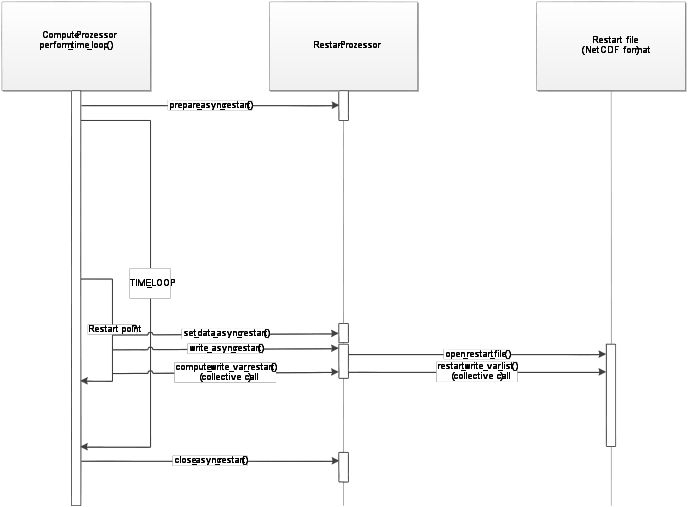
\includegraphics[width=\textwidth]{ICONImplementierungAsynchronerRestart-img001.png}
 \caption{Sequenzdiagramm des asynchronen Restarts}
\end{figure} 


\section{Ausblick}

Die Schreibfunktionalit\"at wurde bereits vorbereitet, dass bei paralleler Ausgabe mehrerer ICON-Patches durch mehrere
Restart-Prozessoren die erzeugten Restart-Dateien im Namen um den Wert eines Z\"ahlers erweitert werden.
Um diese Funktionalit\"at verwenden zu k\"onnen, muss aber noch die Import-Seite codem\"a\ss ig angepasst werden, damit die
erzeugten Restart-Dateien wieder entsprechend eingelesen werden.
Zum Zeitpunkt der Entwicklung des asynchronen Restarts wurde durch den Restart-Import nur eine Restart-Datei importiert.\\

Im Vergleich zum synchronen Restart m\"ussen die Compute-Prozessoren nicht darauf warten bis der zugeh\"orige Restart-Prozessor
seine Daten in die Restart-Datei ausgegeben hat, sondern k\"onnen unmittelbar mit Ihren Berechnungen fortfahren, sobald sie
ihre Daten in einem vom Restart-Prozessor eingerichteten Speicher-Bereich geschrieben haben.\\

Die Restart-Prozessoren lesen die Restart-Variablen aus diesem Speicherbereich und schreiben sie in ein oder mehrere
Restart-Dateien, w\"ahrend die Compute-Prozessoren bereits weitere Berechnungen durchf\"uhren.
Zeitlich begrenzt wird der beschriebene Vorgang nur dadurch, dass die Restart-Prozessoren ihre Arbeit erst beendet
haben m\"ussen, bevor sie f\"ur eine weitere Restart-Ausgabe zur Verf\"ugung stehen.\\

M\"ussen Compute-Prozessoren auf die Beendigung der Restart-Ausgaben warten, bis sie einen weiteren Zeitschritt exportieren k\"onnen,
sollte die Anzahl der verwendeten Restart-Prozessoren erh\"oht werden.

\begin{figure}
 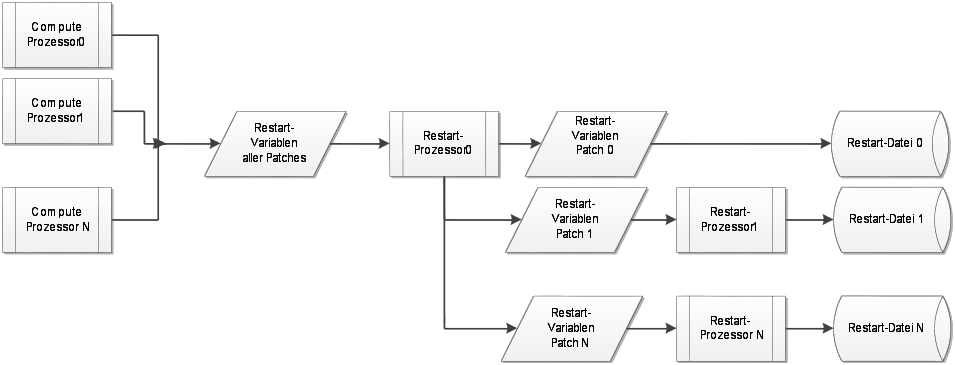
\includegraphics[width=\textwidth]{ICONImplementierungAsynchronerRestart-img002.png}
 \caption{Datenfluss beim asynchronen Schreiben der Restart-Dateien}
\end{figure} 

Bei der Implementierung des asynchronen Restarts wurden folgende Fortran-Dateien ge\"andert bzw. neu erstellt:
\begin{enumerate}
 \item src/drivers/mo\_atmo\_model.f90
 \item src/atm\_dyn\_iconam/mo\_nh\_stepping.f90
 \item src/atm\_dyn\_icoham/mo\_ha\_stepping.f90
 \item src/parallel\_infrastructure/mo\_mpi.f90
 \item src/configure\_model/mo\_parallel\_config.f90
 \item src/io/mo\_io\_restart\_namelist.f90
 \item src/io/mo\_io\_restart\_async.f90
 \item src/namelists/mo\_parallel\_nml.f90
\end{enumerate}

\end{document}
